\documentclass[a4paper, 12pt]{report}
\usepackage[utf8]{vietnam}
\usepackage{amsmath}
\usepackage{amsfonts}
\usepackage{amssymb}
\usepackage{amsthm}
\usepackage{fancyhdr}
\usepackage{mathrsfs}
\usepackage[left=3.5cm,right=2cm,top=3.5cm,bottom=3cm]{geometry}
\usepackage{graphicx}
\usepackage{tikz}
\usepackage{float}
\usepackage{pdfpages}
\usepackage{eufrak}
\usepackage{listings}
\usepackage{tabu}
\renewcommand{\baselinestretch}{1.5}
\setlength{\parindent}{0pt}
\pagestyle{plain}
\pagestyle{fancy}
%\documentclass{article}
%\usepackage{indentfirst}
\usepackage{graphicx}
\usepackage{enumitem}

\usepackage[vietnamese=nohyphenation]{hyphsubst}
\usepackage[vietnamese]{babel}
%\setlength{\parindent}{1cm} % Default is 15pt.

\usepackage{titlesec}

\titleformat*{\section}{\LARGE\bfseries}
\titleformat*{\subsection}{\Large\bfseries}
\titleformat*{\subsubsection}{\large\bfseries}
\titleformat*{\paragraph}{\large\bfseries}
\titleformat*{\subparagraph}{\large\bfseries}

%\newtheorem{theorem}{Định lý}[section]

%\newtheorem*{theorem}{Định lý}[section]
%\newtheorem{theorem}{Theorem}
\usepackage{amsthm}

\newtheorem*{theorem}{Định lý } %without numbering
\newtheorem*{corollary}{Hệ quả } %without numbering
\newtheorem{theoremnum}{Định lý } %without numbering

% \newtheorem{theorem}{Theorem}  %with numberring

\newtheorem{Proposition}{Mệnh đề } %without numbering
\newtheorem*{Propositionproof}{Chứng minh mệnh đề 1: } %without numbering
\newtheorem{claim}{Khẳng định}
\lfoot{\textit{Lai Đức Thắng}}

\rfoot{\textit{Toán Tin K61}}
\renewcommand{\footrulewidth}{1,2pt}



\begin{document}



	\begin{titlepage} % Đây là trang bìa


			\begin{center}
				
				{\large\bf TRƯỜNG ĐẠI HỌC BÁCH KHOA HÀ NỘI}\\
				
				{\large\bf VIỆN TOÁN ỨNG DỤNG VÀ TIN HỌC} \\
				
				{———————o0o——————–}
				\vskip 1cm
%			\includegraphics[scale=0.3]{Logo_Hust}
				\begin{center}
     				
\includegraphics[scale=.85]{biaDA.png}
				\end{center}
				\vskip 1cm
				
%				{\Large\bf \textbf{PHƯƠNG PHÁP\\ 
%						PHÂN TÍCH THÀNH PHẦN CHÍNH\\
%						(Principal Component Analysis - PCA )
%				}}

				{\Large\bf \textbf{VĨNH THỨC
						VÀ ỨNG DỤNG TRONG\\ BÀI TOÁN ĐẾM TỔ HỢP\\
				}}
				\vskip 1cm
				{\bf ĐỒ ÁN III}
				
				
				{\bf {\it Chuyên ngành:} TOÁN TIN}\\
				{\bf {\it Chuyên sâu:} }Xác suất rời rạc
				
				\vskip 1cm
				
				\begin{tabular}{r l}
					
					Giảng viên hướng dẫn:&{\bf TS. TRẦN MẠNH TUẤN }\\[0.5cm]
					
					Họ và tên sinh viên:&{\bf LAI ĐỨC THẮNG}\\[0.5cm]
					
					Số hiệu sinh viên:&{\bf 20163830}\\[0.5cm]
					Lớp:&{\bf Toán Tin K61}
					
				\end{tabular}
				
				\vfill
				
				{\bf HÀ NỘI - 2020}
				
			\end{center}
			
	\end{titlepage}

%\begin{titlepage}
%\begin{center}
%	\textbf{NHẬN XÉT CỦA GIẢNG VIÊN HƯỚNG DẪN}
%\end{center}
%\textbf{1. Mục đích và nội dung của đồ án:}\\
%
%\dotfill
%
%\dotfill
%
%\dotfill
%
%\dotfill
%\\
%\textbf{2. Kết quả đạt được:}\\
%
%\dotfill
%
%\dotfill
%
%\dotfill
%\\
%\textbf{3. Ý thức làm việc của sinh viên:}\\
%
%\dotfill
%
%\dotfill
%
%\dotfill
%
%\dotfill
%\\
%\vskip0.2cm
%\begin{tabular}{ c c}
%	\hspace{7.5cm}    &  {Hà Nội, ngày \quad tháng \quad năm 2020} \\
%	& {Giảng viên hướng dẫn} \\
%		& \textit{(Kí và ghi rõ họ tên)} \\
%\end{tabular}
%\end{titlepage}
%$\mathscr{ABCDEFGHIJKLMNOPQRSTUVWXYZ}$
%$\mathcal{M}$
\tableofcontents
\addcontentsline{toc}{chapter}{Lời mở đầu}

\chapter*{Lời mở đầu}

Để xác định các tính chất của một ma trận, sẽ rất hữu ích khi ta nghiên cứu một số hàm liên quan đến các thành phần của một ma trận. Do đó, trong báo cáo đồ án III này, em xin trình bày về một trong những hàm đó, vĩnh thức, các tính chất, bất đẳng thức liên quan đến vĩnh thức của một ma trận và áp dụng để giải quyết bài toán đếm tổ hợp: xác định số hình vuông Latin bậc n.
Bố cục của đồ án “Vĩnh thức và ứng dụng trong bài toán đếm tổ hợp” bao gồm:
\begin{itemize}
	\item \textbf{Chương 1: Vĩnh thức}
		\par \setlength{\parindent}{5ex} Khái niệm vĩnh thức của ma trận M (ký hiệu: per(M)) và chứng minh phỏng đoán của Van der Waerden để tìm chặn dưới phù hợp cho vĩnh thức.

	\item \textbf{Chương 2: Lý thuyết thông tin} 
	\par \setlength{\parindent}{5ex} Trình bày kiến thức cơ sở lý thuyết về thông tin và độ đo cơ bản của thông tin là Entropy; khái niệm về entropy có điều kiện và một số quan hệ giữa các đại lượng trong entropy có điều kiện

	\item \textbf{Chương 3: Entropy trong bài toán Vĩnh thức}
	\par \setlength{\parindent}{5ex} Nhắc lại các khái niệm cơ bản về đồ thị, đồ thị hai phía, mối liên hệ giữa ma trận M/{0,1} và đồ thị hai phía: số lượng các ghép cặp hoàn hảo = per(M), từ đó sử dụng entropy từ lý thuyết thông tin để chứng minh một định lý về vĩnh thức của  Brégman, thông qua đó xác định được một chặn trên phù hợp cho giá trị này.
	\item \textbf{Chương 4: Hình vuông Latin}
	\par \setlength{\parindent}{5ex} Giới thiệu hình vuông Latin và ứng dụng của vĩnh thức trong bài toán tổ hợp tìm số hình vuông Latin bậc n. \\ 
	Em xin chân thành cảm ơn thầy Trần Mạnh Tuấn đã trực tiếp hướng dẫn và chỉ ra những điểm còn thiếu sót trong bài để em nhanh chóng khắc phục và hoàn thành bài báo cáo một cách tốt nhất.
	Do kiến thức còn hạn hẹp không tránh khỏi những thiếu sót trong cách hiểu và trình bày. Em rất mong nhận được sự đóng góp ý kiến của quý thầy cô để bản báo cáo của em đạt được kết quả tốt hơn.
	Em xin chân thành cảm ơn!



\end{itemize}





\hspace*{9cm}\textit{Hà Nội, tháng 6 năm 2020}
	
\hspace*{9.5cm}\text{Sinh viên thực hiện}
	
\hspace*{10cm}\text{Lai Đức Thắng}

\chapter{Vĩnh thức}
Nội dung chính của chương này dựa theo chương 24 của cuốn sách ‘‘Proofs from THE BOOK’’, Martin Aigner, Günter M. Ziegler, , $6^{th}$ Edition.
\section{Khái niệm}
Giả sử $M= (m_{ij})$ là ma trận số thức $n \times n$. Khi đó vĩnh thức (Permanents) của ma trận $M$ (kí hiệu là $per$):
\begin{equation*}
per M = \displaystyle \sum_{\sigma \in S_{n}}m_{1\sigma(1)}m_{2\sigma(2)}...m_{n\sigma(n)}
\end{equation*}
trong đó $S_{n}$ là tập tất cả các hoán vị của $\{1,2,...,n\}$.
\section{Phỏng đoán của Van der Waerden}
Khác với định thức, có thể tính toán nhanh chóng (sử dụng phép khử Gauss ), việc tính toán với vĩnh thức là khá khó khăn. Một vài nghiên cứu gần đây về vĩnh thức xem xét về xấp xỉ và giới hạn của giá trị này. Trong nội dung bài báo cáo này ta xem xét đến một định lý nổi tiếng về vĩnh thức và chứng minh của nó. Một ma trận $M=(m_{ij})$ được gọi là \textit{ngẫu nhiên kép} (\textit{doubly stochastic}) nếu các phần tử của ma trận là các số thực không âm sao cho tổng theo mỗi hàng hoặc mỗi cột bằng $1$. Năm 1926 Bartel L. Vander Waerden đưa ra phỏng đoán: 
\begin{equation*}
\textrm{per } M \geq \frac{n!}{n^n}
\end{equation*}
đúng với mọi ma trận \textit{ngẫu nhiên kép} $n \times n $ . Dấu "$=$"  xảy ra khi và chỉ khi $M=(m_{ij})$, trong đó $m_{ij} = \frac{1}{n}$ với mọi $i$ và $j$
Phỏng đoán này chưa được giải quyết trong hơn 50 năm, cho đến khi được xác nhận bởi G. P. Egorchev và D. I. Falikman vào băn 1981. Sau đó, vào năm 2007, Leonid Gurvits đưa ra một chứng minh ngắn gọn và hoàn toàn khác biệt. Trước hết ta sẽ phát biểu lại định lý.
\begin{theoremnum}
Đặt $M=(m_{ij})$ là ma trận \textit{ngẫu nhiên kép} $n \times n $. Khi đó
\begin{equation}
\textrm{per } M \geq \frac{n!}{n^n} \label{eqPer}
\end{equation}
Dấu "$=$" xảy ra khi và chỉ khi  $m_{ij} = \frac{1}{n}$ với mọi $i$ và $j$.
\end{theoremnum}
Đầu tiên ta sẽ chuyển ma trận về dạng đa thức. Với mọi ma trận $n  \times n$ $M = (m_{ij}) $, ta xây dựng một đa thức $p_M(x) \in R_{[x_1,...,x_n]} $, 
\begin{equation*}
	p_M(x) = p_M(x_1,..,x_n) := \displaystyle \prod_{i=1}^{n} \Big( \displaystyle \sum_{j=1}^{n} m_{ij}x_j \Big).
\end{equation*}
Tiếp theo ta định nghĩa đạo hàm của $p_M(x) \in R_{[x_1,...,x_n]} $  theo biến $x_n$:
\begin{equation*}
	 p'(x_1,..,x_{n-1}) := \frac{\partial p(x)}{\partial x_n}\mid _{x_n = 0}
\end{equation*}
Quan sát rằng $p$ là đa thức thuần nhất bậc $n$ với $n$ biến, khi đó $p'$ là đa thức thuần nhất bậc $n-1$ với $n-1$ biến. Tổng quát, với $i=0,1,..,n$
\begin{equation*}
	 q_i(x_1,..,x_{i}) := \frac{\partial^{n-i} p(x)}{\partial x_n...\partial x_{i+1}}\mid _{x_n = x_{n-1} = ... = x_{i+1} = 0}
\end{equation*}
Từ công thức trên ta nhận được một dãy $(q_n,q_{n-1},...,q_0)$, trong đó $q_n=p$ và $q_{i-1} = q_{i}'$ với $1 \leq i \leq n$ và $q_0$ là hệ số của $x_1x_2...x_n$ trong đa thức $p$. Thêm nữa, nếu $p$ là đa thức thuần nhất bậc $n$, thì $q_i$ là đa thức thuần nhất bậc $q_i$. Xét dãy sinh ra bởi đa thức $p_M(x)$,
\begin{equation*}
p_M(x) = q_n,...,q_i,...,q_0
\end{equation*}
Ta suy ra hai điều quan trọng sau đây: 
\begin{enumerate}[label=\textbf{\Alph*.}]
\item $per$ $M$ là hệ số của $x_1x_2...x_n$ trong $q_n$, do đó $q_0 = \textrm{per }M$.
\item Với  $i=1,..,n$ ta có
\begin{equation}
	deg_{i}q_i \leq min\{i,\lambda_M(i)\}, \label{deg}
\end{equation}
trong đó $deg_{i}q_i $ kí hiệu là bậc của $x_{j}$ trong $q_i(x_1,...,x_n)$ và $\lambda_M(i)$ là số các giá trị khác 0 trong cột thứ $i$ của ma trận $M$. \\
Thật vậy, ta có $deg_{i}q_i \leq i$ vì $q_i$ là đa thức thuần nhất bậc $i$, trong khi $deg_{i}q_i \leq deg_{i}q_n \leq \lambda_M(i)$ là hiển nhiên theo định nghĩa của $p_M(x)$.
\end{enumerate}
Sau đây là ý tưởng chính của chứng minh: Ta liên kết một tham số với mỗi đa thức $p$ và xác định một cận dưới cho tham số đó khi truyền từ $p$ sang $p'$.\\
Ta kí hiệu $\mathbb{R}_{+}$ là tập các số thực không âm và $p(x) \in \mathbb{R}_{+[x_1,...,x_n]}$ là đa thức trong đó các hệ số của $p(x)$ là không âm. Với số thức $z \in \mathbb{C}$, đặt $Re(z)$ và $Im(z)$ lần lượt là phần thực và phần ảo của $z$. Đặt $\mathbb{C}_{+} = \{z \in \mathbb{C}: Re(z) \geq 0\}$ và $\mathbb{C}_{++} = \{z \in \mathbb{C}: Re(z) > 0\}$. Kí hiệu này mở rộng với $\mathbb{R}_{+}^{n}$ và $\mathbb{C}_{+}^{n}$. Ví dụ, $z=(z_1,...,z_n) \in \mathbb{C}_{++}^{n}$ đúng nếu $Re(z_i) >0$ với mọi $i$.\\
Với mọi đa thức $p(x) \in \mathbb{R}_{+[x_1,...,x_n]}$ ta định nghĩa \textbf{capacity} của $p$, kí hiệu $cap(p)$ bởi:
\begin{equation*}
\textrm{cap}(p) := \textrm{inf }\{p(x): x \in \mathbb{R}_{+}^{n}, \displaystyle \prod_{i=1}^{n}x_i = 1 \}
\end{equation*}
Đặc biệt cap($p$) $\geq 0$ vì p chỉ có các hệ số không âm, và nếu $p$ là hằng số ($p(x) \equiv c$) thì cap($p$) $= c$
Ngoài ra ta cần hàm $g: \mathbb{N}_{0} \rightarrow \mathbb{R}$ với $g(0) :=1$ và 
\begin{equation*}
	g(k) := \Big( \frac{k-1}{k} \Big)^{k-1}  \textrm{                   với    } k \geq 1.
\end{equation*}
Sử dụng bất đẳng thức $1 +x \leq e^x$ 2 lần, ta được
\begin{equation*}
	\frac{g(k+1)}{g(k)} = \frac{k}{k+1} \Big( \frac{k^2}{k^2 - 1}\Big) ^{k-1} < e^{-\frac{1}{k+1}}e^{\frac{1}{k^2 - 1}} =1
\end{equation*}
với $k \geq 1$. Do đó, $g$ là hàm không tăng, $g(0) = g(1) > g(2) > ...$ .\\
Ta gọi đa thức $p(x) \in \mathbb{R}_{[x_1,...,x_n]}$ là \textit{H-ổn định} nếu đa thức này không có nghiệm trên $C_{++}^{n}$.

\textbf{Mệnh đề Gurvits}
\textit{Nếu $p(x) \in \mathbb{R}_{+[x_1,...,x_n]}$ là H-ổn định và thuần nhất bậc $n$, khi đó hoặc $p' \equiv 0$ hoặc $p'$ là H-ổn định và thuần nhất bậc $n-1$. Trong cả hai trường hợp}
\begin{equation}
 \textrm{cap}(p') \geq \textrm{cap}(p).g(\textrm{deg}_{n}p) \label{Gurvits}
\end{equation}
\textbf{Chứng minh Định lý 1.}
Đặt $M=(m_{ij})$ là ma trận \textit{ngẫu nhiên kép} $n \times n$. Ta đã biết $p_M(x)$ là đa thức thuần nhất bậc n. Khi đó hai khẳng định dưới đây là đúng:
\begin{claim}
	$p_M(x)$ là H-ổn định
\end{claim}
Bằng phản chứng, giả sử $x$ là nghiệm của $p_M(x)$. Từ $p_M(x) = \prod_{i=1}^{n} (\sum_{j=1}^{n} m_{ij}x_{j}) =0$ suy ra $\sum_{j=1}^{n} m_{ij}x_{j} =0$ nên $\sum_{j=1}^{n} m_{ij}Re(x_{j}) =0$. Điều này trái với giả thiết $x \in \mathbb{C}^{n}_{++}$, vì $m_{il} > 0$ với một vài giá trị $l$. 
\begin{claim}
	$\hbox{cap}(p_M)$
	$cap(p_M) =1$
\end{claim}
\begin{proof}
	Trước tiên ta nhắc lại bất đẳng thức $AM-GM$: Với $a_1,...,a_n, p_1,..,p_n \in \mathbb{R}_{+}$ thoả mãn $\sum_{i=1}^{n}p_{i} =1$ ta có
	\begin{equation}
		\displaystyle \sum_{i=1}^{n} p_{i}a_{i} \geq a_{1}^{p_1}...a_{n}^{p_n}. \label{amgm}
	\end{equation}
Chọn bất kì giá trị $x \in \mathbb{R}_{+}^{n}$ với $\prod_{j=1}^{n}x_{j} =1$. Áp dụng bất đẳng thức AM-GM:
\begin{equation*}
\begin{array}{l@{}l}
	p_M(x) = \displaystyle \prod_{i=1}^{n} \Big( \displaystyle \sum_{j=1}^{n} m_{ij}x_{j} \Big) &{}\geq \displaystyle \prod_{i=1}^{n} \displaystyle\prod_{j=1}^{n} x_{j}^{m_{ij}} \\
	&{}= \displaystyle\prod_{j=1}^{n}\displaystyle \prod_{i=1}^{n}x_{j}^{m_{ij}} = \displaystyle\prod_{j=1}^{n} x_j^{\sum_{i=1}^{n} m_{ij}} \\
	&{}= \displaystyle\prod_{j=1}^{n} x_j =1
\end{array}
\end{equation*}
do đó $cap(p_M) \geq 1$. \\
Mặt khác,
\begin{equation}
	p_M(1,1,...,1) = \displaystyle \prod_{i=1}^{n} \Big (\displaystyle \sum_{j=1}^{n} m_{ij} \Big) = \displaystyle\prod_{i=1}^{n} 1 =1,
\end{equation}
\end{proof} 
Vì $p_M(x)$ là \textit{H-ổn định}, ta có thể áp dụng mệnh đề \eqref{Gurvits} nhiều lần để đưa ra kết luận mọi đa thức $q_i$ đều là \textit{H-ổn định}, sao cho với mỗi giá trị của $i$:
\begin{equation}
	cap(q_{i-1}) \geq cap(q_i)g(deg_{i}q_i) \geq cap(q_i)g(min \{i, \lambda_{M}(i)\}), \label{iterate}
\end{equation}
trong đó bất đẳng thức thứ hai được suy ra từ \eqref{deg} với $g$ là hàm giảm.\\ 
Lặp lại  \eqref{iterate}   bắt đầu với $cap(p_M) =1$, ta có:
\begin{equation*}
\begin{array}{l@{}l}
	per M 
	= q_0 &{}\geq \displaystyle \prod_{i=1}^{n} g(min \{i,\lambda_M(i) \} )\\
	&{}\geq \displaystyle \prod_{i=1}^{n}g(i) = \displaystyle \prod_{i=1}^{n} \Bigg( \frac{i-1}{i} \Bigg)^{i-1} = \displaystyle \prod_{i=1}^{n}i\frac{(i-1)^{i-1}}{i^i} = \frac{n!}{n^n}
\end{array}
\end{equation*} \qed




%\chapter{Entropy và bài toán vĩnh thức}
\chapter{Lý thuyết thông tin}
\section{Khái niệm}
Lý thuyết thông tin (Information Theory) là một nhánh toán ứng dụng quan tâm đến các vấn đề định lượng (quantification), lưu trữ (storage) và truyền thông (communication) của thông tin.Lý thuyết thông tin được khởi xướng bởi Claude E. Shannon vào năm 1948 với bài báo khoa học có tiêu đề “A Mathematical Theory of Communication” đặt nền móng nghiên cứu nền tảng về các giới hạn liên quan đến xử lí tín hiệu (signal processing) và các thao tác truyền thông (communication operations) như nén dữ liệu. Phần lớn ứng dụng của lý thuyết thông tin thường liên quan đến việc nén dữ liệu (ZIP, MP3, JPEG,…) và mã hóa kênh (truyền dữ liệu số qua đường dây điện thoại,…).


\section{Entropy}
Trong lý thuyết thông tin, một độ đo cơ bản của thông tin là entropy, thường được diễn đạt dưới dạng số lượng bit cần thiết trung bình để lưu trữ hoặc dẫn truyền. Entropy lượng hóa sự không chắc chắn trong việc dự đoán giá trị của một biến ngẫu nhiên. Ví dụ như, xác định kết quả của một lần tung đồng xu công bằng (hai kết quả có khả năng như nhau) cho ít thông tin hơn (entropy nhỏ hơn) là xác định kết quả của một lần tung xúc sắc (sáu kết quả có khả năng như nhau).\\
Giả sử X là một biến ngẫu nhiên nhận các giá trị $\{a_{1},...,a_{n}\}$ với xác suất $Pr(X=a_{i}) = p_{i}$. Nó giúp ta suy nghĩ về việc coi $X$ là một phép thử với các khả năng là $a_{i}$, giống như việc tung một xúc xắc với các khả năng là số chấm trên xúc xắc đó ${1,2,3,4,5,6}$. Vậy lượng thông tin (về trung bình) nhận được từ phép thử trên là bao nhiêu? 

Với biến ngẫu nhiên rời rạc  $X$ nhận các giá trị $\mathscr{X}=\{x_{1},...,x_{n}\}$ và hàm phân phối xác suất $Pr(X)$ thì Entropy của $X$ là:
\begin{equation*}
H(X) = \displaystyle \sum_{i=1}^{n}Pr(x_i)\log_{b}\frac{1}{Pr(x_i)},
\end{equation*}
trong đó ta quy ước $0.log(\frac{1}{0}) = 0$ (giả định rằng tổng chỉ được lấy trên các phần tử $x \in \mathscr{X}$ sao cho $Pr(X=x)>0$). Khi đó \textit{giá}($support$) của biến ngẫu nhiên $X$ là: $supp\textrm{ }X := \{a: Pr(X=a) > 0\}$. Biểu thức trên cũng có thể được viết lại thành: 
\begin{equation*}
H(X) = -\displaystyle \sum_{i=1}^{n}Pr(x_i)\log_{2}Pr(x_i)
\end{equation*}
Đôi lúc để ký hiệu tiện lợi và dễ nhìn hơn chúng ta có thể viết lại công thức Entropy với vector xác suất $p=(p_i,...,p_n)$ với $p_i = Pr(X=x_i)$. Khi đó:
\begin{equation*}
H(X) = -\displaystyle \sum_{i=1}^{n}p_i\log_{2}p_i
\end{equation*}
Xét một ví dụ, nếu X là sự kiện tung một đồng xu với $Pr(X = \textrm{ngửa}) = p$, khi đó theo công thức của Shannon cho ta hàm $H(X_{p,1-p}) = -p\log_{2}p-(1-p)\log_{2}(1-p)$ 
%(hình \ref{fig:t}).
%\begin{figure}
%\begin{center}
%	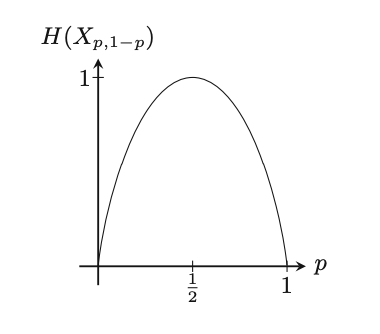
\includegraphics[width=7cm]{funcEntropy}\\
%	\caption{}
%	\label{fig:t}
%\end{center}
%\end{figure}
\section{Entropy có điều kiện}
Giả sử $X$ và $Y$ là hai biến ngẫu nhiên nhận các giá trị lần lượt $\{a_1,..,a_m\}$ và $\{b_1,..,b_n\}$. Entropy hợp (\textit{joint entropy}) của 2 biến ngẫu nhiên $X$ và $Y$ là:
\begin{equation*}
H(X,Y) = -\displaystyle \sum_{i=1}^{n}p_i\log_{2}p_i
\end{equation*}

Nếu \(p(b_{j}|a_{i}):= Pr(Y=b_{j}|X=a_{i})\) là xác suất có điều kiện của $b_j$ khi biết $a_i$. Khi đó entropy có điều kiện của \(Y\)nếu ta biết kết quả của \(X\) là \(a_{i}\) là:
\begin{equation*}
    H(Y|a_{i}) := -\sum_{i=1}^{n}p(b_{j}|a_{i})\log_{2}p(b_{j}|a_{i})
\end{equation*}
Nếu lấy giá trị kì vọng của biểu thức trên với tất cả các khả năng của X, ta thu được:
\begin{equation*}
    H(Y|X) := \sum_{i=1}^{n}p(a_{i})H(Y|a_{i})
\end{equation*}
chính là entropy có điều kiện của $Y$ khi biết $X$
Sau đây ta sẽ xem một số mối quan hệ giữa các đại lượng ở trên.
\begin{Proposition}
Giả sử $X$ và $Y$ là hai biến ngẫu nhiên nhận các giá trị trong tập $\mathscr{X}$ và $\mathscr{Y}$. Ta có một số kết quả sau:
\end{Proposition}
\begin{enumerate}[label=\textbf{(\Alph*)}]
\item \(H(X) \leq \log_{2}(|supp X|)\). Dấu "$=$"  xảy ra khi và chỉ khi $X$ là phân phối đều trên $supp \textrm{ X}$, tức $Pr(X=a) = \frac{1}{n}$ với $a \in \textrm{supp }X$, $n=|\textrm{supp }X|$
\item \(H(X,Y) = H(X) + H(Y|X)\), và tổng quát ta có \(H(X_{1},...,X_{n}) = H(X_{1}) + H(X_{2}|X{1}) + ... + H(X_{n}|X_{1},...,X_{n-1})\).
\item \(H(X,Y) \leq H(X) + H(Y|X)\) . Dấu "$=$" xảy ra khi và chỉ khi $X$ và $Y$ là độc lập.
%\item \(H(X,Y) \leq H(X) \).
\item Nếu \(supp\) \(X\) được chia thành $d$ tập \(E_{1},..,E_{d}\) sao cho \(E_{j}:= \{a \in suppX : |supp(Y|a)| = j \} \) thì:
\begin{equation*}
    H(Y|X) \leq \sum_{j=1}^{d}Pr(X \in E_{j})\log_{2}j.
\end{equation*}
\end{enumerate}
%Trước khi đi vào chứng minh, ta nhắc lại bất đẳng thức $AM-GM$: 
%\begin{equation*}
%	a_{1}^{p_{1}}. ... .a_{n}^{p_{n}} \leq p_{1}a_{1}. ... .p_{n}a_{n}
%\end{equation*}

\begin{proof}[Chứng minh mệnh đề 1]\textit{ }
\begin{enumerate}[label=(\Alph*)]
\item Không mất tính tổng quát, giả sử $p_{i} > 0$  $\forall i$. Áp dụng bất đẳng thức \textbf{AM-GM} \eqref{amgm}: Đặt $a_{i} = \frac{1}{p_{i}}$ và lấy $\log$ 2 vế, ta được:
\begin{equation*}
H(X) = \displaystyle \sum_{i=1}^{n}p_{i}\log_{2}\frac{1}{p_{i}} \leq \log_{2}\Big(\displaystyle \sum_{i=1}^{n}p_{i}\frac{1}{p_{i}}\Big) = \log_{2}n.
\end{equation*}
Dấu "$=$" xảy ra khi và chỉ khi $p_{1} = ... = p_{n} = \frac{1}{n}$.

\item 

\begin{equation*}
\begin{array}{l@{}l}
H(X,Y)
	&{}= \displaystyle -\sum_{i,j}p(a_{i},b_{j})\log_{2} p(a_{i},b_{j}) \\
	&{}= \displaystyle -\sum_{i,j}p(a_{i},b_{j})\log_{2} p(a_{i})p(b_{j}|a_{i}) \\ 
	&{}= \displaystyle -\sum_{i,j}p(a_{i},b_{j})[\log_{2}p(a_{i}) + \log_{2}p(b_{j}|a_{i}) ] \\
	&{}= \displaystyle -\sum_{i,j}p(a_{i},b_{j})\log_{2}p(a_{i})  \displaystyle -\sum_{i,j}p(a_{i},b_{j})\log_{2}p(b_{j}|a_{i}) \\
	&{}= \displaystyle -\sum_{i,j}p(a_{i},b_{j})\log_{2}p(a_{i}) \displaystyle -\sum_{i,j}p(a_{i}).p(b_{j}|a_{i})\log_{2}p(b_{j}|a_{i}) \\
	&{}= \displaystyle -\sum_{i=1}^{m}p(a_{i}) \log_{2}p(a_{i}) \displaystyle \sum_{j=1}^{n}p(b_{j}|a_{i}) + H(Y|X) \\
	&{}= \displaystyle -\sum_{i=1}^{m}p(a_{i}) \log_{2}p(a_{i}) + H(Y|X) = H(X) + H(Y|X) .
\end{array}.
\end{equation*}
(Do $\displaystyle \sum_{j=1}^{n}p(b_{j}|a_{i}) = \displaystyle \sum_{j=1}^{n}\frac{P(b_{j}.a_{i})}{P(a_{i})} = \frac{1}{P(a_{i})}\displaystyle \sum_{j=1}^{n}P(b_{j}.a_{i})=\frac{1}{P(a_{i})}P(a_{i}) =1  $)
\item Vì $Pr(X=x) = \displaystyle \sum_{y \in \mathscr{Y}}Pr(X=x,Y=y)  $,\\
$H(X) + H(Y) = \displaystyle -\sum_{x,y}Pr(X=x,Y=y)\log(Pr(X=x).Pr(Y=y)) $.sử dụng bất đẳng thức ...., ta có:
\begin{equation*}
\begin{array}{l@{}l}
H(X,Y) - (H(X) + H(Y)) 
	&{}= \displaystyle \sum_{x,y}Pr(X=x,Y=y)\log\Bigg(\frac{Pr(X=x).Pr(Y=y)}{Pr(X=x,Y=y)}\Bigg) \\
	&{}\leq \log \Bigg( \displaystyle \sum_{x,y}Pr(X=x).Pr(Y=y)\Bigg)\\
	&{}= \log 1 =0 
\end{array}
\end{equation*}
Dâu "$=$" xảy ra khi và chỉ khi $X$,$Y$ độc lập với nhau.
%\item Theo $(B)$ và $(C)$:
%\begin{equation*}
%	H(Y|X) - H(X) = H(X,Y) - H(Y) - H(X) \leq 0,
%\end{equation*}
Dấu "$=$" xảy ra  khi và chỉ khi $X$,$Y$ độc lập với nhau.

\item Ta có $supp\textrm{ }(Y|a) = \{b: Pr(Y=b|X=a) > 0 \}$ .Vì $Pr(Y=b|X=a)$ là 1 biến ngẫu nhiên trên tập $supp$ $(Y|a)$ (Do $\displaystyle \sum_{i=1}^{m}Pr(Y=b_{i}|a) =1$) Tiến hành chia tập $supp$ $X$ thành các tập con $E_{j}$ theo giả thuyết và sử dụng kết quả từ \textbf{(A)}, ta có:
%$H(Y|X) = \displaystyle \sum_{i=1}^{m}p(a_{i})H(Y|a_{i}) $.  

\begin{equation*}
\begin{array}{l@{}l}
H(X,Y)
	&{} = \displaystyle \sum_{i=1}^{m}p(a_{i})H(Y|a_{i}) \\
	&{}= \displaystyle \sum _{j=1}^{d}\sum_{a \in E_{j}}p(a)H(Y|a) \\
	&{} \leq \displaystyle \sum _{j=1}^{d}\sum_{a \in E_{j}}p(a)\log_{2}j \\
	&{} = \displaystyle \sum_{j=1}^{d}Pr(X \in E_{j})\log_{2}j.
\end{array}
\end{equation*}
\end{enumerate}
\end{proof}



\chapter{Entropy và bài toán Vĩnh thức}
Nội dung chính của chương này dựa theo chương 37 của cuốn sách ‘‘Proofs from THE BOOK’’, Martin Aigner, Günter M. Ziegler, , $6^{th}$ Edition.\\
Trước khi đi vào nội dung chương này, em xin nhắc lại một số định nghĩa cơ bản và thuật ngữ về đồ thị. Một đồ thị $G = (V,E)$ là một cấu trúc bao gồm tập hữu hạn các \textit{đỉnh} $V$ (hay được gọi là các \textit{nút}) và tập hợp hữu hạn các \textit{cạnh} $E$ sao cho mỗi \textit{cạnh} $e$ được liên kết với một cặp \textit{đỉnh} $v$ và $w$. Khi hai đỉnh là điểm cuối của một cạnh thì ta nói chúng \textit{kề nhau}. \textit{Lân cận} của một đỉnh là tập các đỉnh kề với đỉnh đó.
\section{Đồ thị hai phía}
\subsection{Khái niệm}
Một đồ thị đơn vô hướng $G: = (V,E)$ được gọi là đồ thị hai phía nếu tồn tại một phân hoạch của tập đỉnh $V=V_1 \cup V_2$ sao cho $V_{1}$ và $V_{2}$ là các tập độc lập và thoả mãn: bất kỳ cạnh nào thuộc tập cạnh $E$ của đồ thị cũng nối một đỉnh $\in V_1$ với một đỉnh $\in V_2$.  Ta thường viết $G: = (V_{1} \cup V_{2},E)$ để ký hiệu một đồ thị hai phía với các phân hoạch $V_1$ và $V_2$. Nếu |$ V_{1} | = | V_{2} |$ thì G được gọi là đồ thị hai phía cân bằng. \\
Ví dụ về đồ thị hai phía: 
\begin{figure}
\begin{center}
	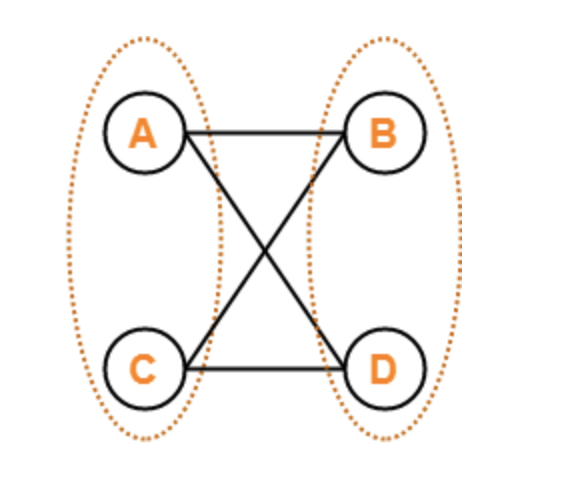
\includegraphics[width=7cm]{ex1}\\
 	\caption{Ví dụ về đồ thị hai phía}
	\label{fig:t}
\end{center}
\end{figure}
Đồ thị (\ref{fig:t}) là một đồ thị hai phía vì:
\begin{itemize}
	\item Các đỉnh của đồ thị có thể phân tách thành hai tập $V_1=\{A,C\}$ và $V_2=\{B,D\}$ 
	\item Các đỉnh của tập $V_1$ chỉ nối với các đỉnh của tập $V_2$ và ngược lại
	\item Các đỉnh trong cùng một tập không kề với nhau 
	\item |$ V_{1} | = | V_{2} | =2$ nên đây là đồ thị hai phía cân bằng
\end{itemize}

Một \textbf{cặp ghép} (matching) trong một đồ thị $G: = (V,E)$ là tập các cạnh $M \subseteq E$ đôi một không có điểm chung. Một đỉnh của đồ thị được gọi là đã ghép (matched) nếu nó là đầu mút của một cạnh trong $M$. Ngược lại, ta gọi đỉnh đó là đỉnh chưa ghép (unmatched). Một cặp ghép được gọi là \textbf{hoàn hảo} (perfect matching) nếu mọi đỉnh của đồ thị đều đã được ghép.
\subsection{Tính chất}
Một đồ thị hai phía có thể được mô tả qua những cách sau: 
\begin{itemize}
	\item Một đồ thị là hai phía khi và chỉ khi nó không chứa chu trình lẻ.
	\item Một đồ thị là hai phía khi và chỉ khi có thể tô màu nó bằng hai màu.
	\item Phổ của đồ thị là đối xứng khi và chỉ khi đó là đồ thị hai phía


\end{itemize}
\subsection{Ứng dụng}
Đồ thị hai phía thường được dùng để mô hình các bài toán ghép cặp (matching problem). Một ví dụ bài toán phân công công việc. Giả sử ta có một nhóm người $P$ và một tập công việc $J$, trong đó không phải ai cũng hợp với mọi công việc. Ta có thể mô hình bài toán bằng một đồ thị với tập đỉnh là $ P + J$. Nếu người $p_i$ có thể làm công việc $j_i$, đồ thị sẽ có một cạnh nối giữa $p_i$ và $j_i$. Định lý hôn nhân cung cấp một đặc điểm của đồ thị hai phía: tồn tại cặp ghép hoàn hảo (perfect matching).

Đồ thị hai phía được sử dụng trong lý thuyết mã hóa (coding theory) hiện đại, đặc biệt khi giải mã các codeword nhận được từ kênh. Đồ thị nhân tử (factor graph) và đồ thị Tanner là các ví dụ.

\section{Định lý Brégman}
\subsection*{Mô hình bài toán}
Xét ma trận $n \times n$ $M =( m_{ij}) $ với các phần tử $\{0,1\}$. Ta liên kết $M$ với một đồ thị hai phía $G_{M} = (U \cup V ,E)$, trong đó $U=\{u_{1},..,u_{n}\}$, $V=\{v_{1},..,v_{n}\}$ thoả mãn: 
\begin{equation*}
    u_{i}v_{j} \in E \Longleftrightarrow m_{ij}=1
\end{equation*}
Ngược lại, mọi đồ thị hai phía G với $n+n$ nút cho ta một ma trận $\{0,1\}$ có kích thước $n \times n$ với $G=G_M$. Xét biểu thức vĩnh thức của ma trận $M$:
\begin{equation*}
	per M = \displaystyle \sum_{\sigma \in S_{n}}m_{1\sigma(1)}m_{2\sigma(2)}...m_{n\sigma(n)}
\end{equation*}
Khi đó, mỗi thành phần $m_{1\sigma(1)}m_{2\sigma(2)}...m_{n\sigma(n)}$ nhận giá trị $0$ hoặc $1$; bằng 1 khi và chỉ khi tập các cạnh $\{u_{1}v_{\sigma(1)},...,u_{n}v_{\sigma(n)}\}$ là một \textit{ghép cặp hoàn hảo (perfect matching)} của $G_M$ và ngược lại. Do đó số lượng \textit{ghép cặp hoàn hảo} $m(G_M)$ chính là giá trị của vĩnh thức, hay $per M = m(G_M)$.
Mối liên hệ giữa $G \leftrightarrow M_G$ đã minh hoạ cho một nghiên cứu về vĩnh thức. Một trong những vẫn đề khó khăn đầu tiên là một phỏng được đưa ra bởi Henryk Minc vào năm 1967: Giả sử ma trận $M$$-\{0/1\}$ có tổng theo hàng $d_1,...,d_n$ (tương đương với các đỉnh $u_1,..u_n$ có bậc $d_1,..d_n$), khi đó:
\begin{equation*}
    per M \leq \prod_{i=1}^{n}(d_{i}!)^{1/d_{i}}.
\end{equation*}
Phỏng đoán trên của Minc được Lev M. Brégman chứng minh vào năm 1973. Một vài năm sau Alexander Schrijver đưa ra một chứng minh khác ngắn hơn. Tuy nhiên, trong nội dung báo cáo này, em xin trình bày lại chứng minh của Jaikumar Radhakrishnan, sử dụng \textit{Entropy từ lý thuyết thông tin.} Trước tiên ta nhắc lại định lý Brégman :

%\begin{theorem}
%Đặt M = ($m_{ij}$) là ma trận cấp $n \times n$ với các phần tử $\{0,1\}$, và đặt $d_{1},...,d_{n}$ là tổng các hàng của ma trận $M$, tức $d_{i} = \sum_{j=1}^{n}m_{ij}$. Khi đó
%\begin{equation*}
%    per M \leq \prod_{i=1}^{n}(d_{i}!)^{1/d_{i}}.
%\end{equation*}
%\end{theorem}
%
%\begin{proof}
%a
%\end{proof}

%Để chứng minh định lý của Bregman, ta sử dụng 3 mệnh đề dưới đây:
%\begin{enumerate}[label=\textbf{(\Alph*)}]
%\item 
%	$H(X) \leq \log_{2}(|supp X|)$. Dấu "$=$" xảy ra khi và chỉ khi X là phân phối đều trên $supp \text{ }X$ (tức $Prob(X=a) = \frac{1}{n}$ với $a \in supp \text{ }X,n=|supp \text{ }X|$.
%\\
%
%\textit{\underline{Chứng minh:}} Không mất tính tổng quát, giả sử $p_{i} > 0$  $\forall i$. Áp dụng bất đẳng thức \textbf{AM-GM}: $a_{1}^{p_{1}}. ... .a_{n}^{p_{n}} \leq p_{1}a_{1}. ... .p_{n}a_{n}$: Đặt $a_{i} = \frac{1}{p_{i}}$ và lấy $\log$ 2 vế, ta được:
%\begin{equation*}
%H(X) = \displaystyle \sum_{i=1}^{n}p_{i}\log_{2}\frac{1}{p_{i}} \leq \log_{2}\Big(\displaystyle \sum_{i=1}^{n}p_{i}\frac{1}{p_{i}}\Big) = \log_{2}n.
%\end{equation*}
%Dấu "$=$" xảy ra khi và chỉ khi $p_{1} = ... = p_{n} = \frac{1}{n}$.
%
%\item 
%	\(H(X,Y) = H(X) + H(Y|X)\), và tổng quát ta có \(H(X_{1},...,X_{n}) = H(X_{1}) + H(X_{2}|X{1}) + ... + H(X_{n}|X_{1},...,X_{n-1})\).
%\\
%
%\textit{\underline{Chứng minh:}}
%\begin{equation*}
%\begin{array}{l@{}l}
%H(X,Y)
%	&{}= \displaystyle -\sum_{i,j}p(a_{i},b_{j})\log_{2} p(a_{i},b_{j}) \\
%	&{}= \displaystyle -\sum_{i,j}p(a_{i},b_{j})\log_{2} p(a_{i})p(b_{j}|a_{i}) \\ 
%	&{}= \displaystyle -\sum_{i,j}p(a_{i},b_{j})[\log_{2}p(a_{i}) + \log_{2}p(b_{j}|a_{i}) ] \\
%	&{}= \displaystyle -\sum_{i,j}p(a_{i},b_{j})\log_{2}p(a_{i})  \displaystyle -\sum_{i,j}p(a_{i},b_{j})\log_{2}p(b_{j}|a_{i}) \\
%	&{}= \displaystyle -\sum_{i,j}p(a_{i},b_{j})\log_{2}p(a_{i}) \displaystyle -\sum_{i,j}p(a_{i}).p(b_{j}|a_{i})\log_{2}p(b_{j}|a_{i}) \\
%	&{}= \displaystyle -\sum_{i=1}^{m}p(a_{i}) \log_{2}p(a_{i}) \displaystyle \sum_{j=1}^{n}p(b_{j}|a_{i}) + H(Y|X) \\
%	&{}= \displaystyle -\sum_{i=1}^{m}p(a_{i}) \log_{2}p(a_{i}) + H(Y|X) = H(X) + H(Y|X)  
%\end{array}
%\end{equation*}
%(Do $\displaystyle \sum_{j=1}^{n}p(b_{j}|a_{i}) = \displaystyle \sum_{j=1}^{n}\frac{P(b_{j}.a_{i})}{P(a_{i})} = \frac{1}{P(a_{i})}\displaystyle \sum_{j=1}^{n}P(b_{j}.a_{i})=\frac{1}{P(a_{i})}P(a_{i}) =1  $)
%
%\item 
%	Nếu \(supp\) \(X\) được chia thành $d$ tập \(E_{1},..,E_{d}\) sao cho \(E_{j}:= \{a \in suppX : |supp(Y|a)| = j \} \) thì:
%\begin{equation*}
%    H(Y|X) \leq \sum_{j=1}^{d}Prob(X \in E_{j})\log_{2}j.
%\end{equation*}
%\\
%\textit{\underline{Chứng minh:}} Ta có $supp(Y|a) = \{b: Prob(Y=b|X=a) > 0 \}$ .Vì $Prob(Y=b|X=a)$ là 1 biến ngẫu nhiên trên tập $supp$ $(Y|a)$ (Do $\displaystyle \sum_{i=1}^{m}Prob(Y=b_{i}|a) =1$) Tiến hành chia tập $supp$ $X$ thành các tập con $E_{j}$ theo giả thuyết và sử dụng kết quả từ \textbf{(A)}, ta có:
%%$H(Y|X) = \displaystyle \sum_{i=1}^{m}p(a_{i})H(Y|a_{i}) $.  
%
%\begin{equation*}
%\begin{array}{l@{}l}
%H(X,Y)
%	&{} = \displaystyle \sum_{i=1}^{m}p(a_{i})H(Y|a_{i}) \\
%	&{}= \displaystyle \sum _{j=1}^{d}\sum_{a \in E_{j}}p(a)H(Y|a) \\
%	&{} \leq \displaystyle \sum _{j=1}^{d}\sum_{a \in E_{j}}p(a)\log_{2}j \\
%	&{} = \displaystyle \sum_{j=1}^{d}Prob(X \in E_{j})\log_{2}j.
%\end{array}
%\end{equation*}
%
%\end{enumerate}





\textbf{Định lý 1.}  Đặt $M = (m_{ij})$ là ma trận $n \times n$ chỉ chứa hai giá trị $\{0,1\}$ và đặt $d_{1},...,d_{n}$  là tổng các hàng của ma trận $M$, hay $d_{i} =  \displaystyle \sum _{j=1}^{n}m_{ij}$. Khi đó:
\begin{equation*}
    per M \leq \prod_{i=1}^{n}(d_{i}!)^{1/d_{i}}.
\end{equation*}

\begin{proof}
 Xét $G=(U \cup V,E)$ là đồ thị hai phía tương ứng với ma trận $M$, trong đó $d_{i}$ là bậc tương ứng của các đỉnh $u_{i}$, và kí hiệu $\mathfrak{S}$ là tập các \textit{perfect matching} của G. Vì $per M=m(G) = |\mathfrak{S}|$ nên thay vì tìm cận trên cho $per M$ như định lý 1, ta sẽ tìm cận trên cho $|\mathfrak{S}|$. Giả sử $|\mathfrak{S}| \neq 0$ và mỗi $\sigma \in \mathfrak{S}$ là một hoán vị tương ứng $\sigma (1) \sigma (2) ....  \sigma (n)$ của các chỉ số. Vì vậy, tương ứng với mỗi giá trị $u_{i} \in U$ là một giá trị $v_{\sigma(i)} \in V$ theo phép song ánh $\sigma$. Ý tưởng ban đầu là chọn $\sigma$ một cách ngẫu nhiên và xét biến ngẫu nhiên $X=(X_{1},X_{2},..,X_{n}) = (\sigma(1),\sigma(2),...,\sigma(n)).$
\\
Theo mệnh đề \textbf{(A)},
\begin{equation*}
H(\sigma (1), \sigma (2), ....  ,\sigma (n)) = \log_{2}(|\mathfrak{S}|)
\end{equation*}

Do đó chỉ cần chỉ ra
\begin{equation}
    H(\sigma(1),...,\sigma(n)) \leq \log_{2}\Big(\prod_{i=1}^{n}(d_{i}!)^{1/d_{i}}\Big) = \sum_{i=1}^{n}\frac{1}{d_{i}}\log_{2}(d_{i}!).
\end{equation}

Tiếp theo, sử dụng mệnh đề \textbf{(B)}, ta có
\begin{equation}
H(\sigma (1), \sigma (2), ....  ,\sigma (n)) = \displaystyle \sum_{i=1}^{n}H(\sigma (i)| \sigma (1), \sigma (2), ....  ,\sigma (i-1)) \label{eqEntropy2}
\end{equation}
Vậy biểu thức entropy có điều kiện ở trên có ý nghĩa gì ? Nó đo mức độ không chắc chắc (\textit{uncertainty}) về đỉnh được ghép với $u_i$ sau khi các tập các đỉnh ghép với $u_1,...,u_{i-1}$ được xác định. Cụ thể, \textit{giá} (\textit{support}) của biến ngẫu nhiên $\sigma(i)$ khi biết $(\sigma(1),...,\sigma(i-1))$ nằm trong tập chỉ số của lân cận $u_i$ mà chưa được ghép với một trong các đỉnh $u_1,...,u_{i-1}$.
\\
Lấy ví dụ, xét đồ thị hai phía (Hình \ref{fig:image1}), có $|\mathfrak{S}| =4$. Vì mọi hoán vị trong $\mathfrak{S}$ là như nhau nên $H(\sigma(1),...,\sigma(4))=\log_{2}4=2$. Khi đó, $H(\sigma(1)) = -\frac{1}{4}\log_{2}\frac{1}{4}-\frac{1}{4}\log_{2}\frac{1}{4} - \frac{1}{2}\log_{2}\frac{1}{2} = \frac{3}{2} $. Tiếp theo, ta sẽ xác định entropy có điều kiện $H(\sigma(2)|\sigma(1))$: Với $\sigma(1) =1 $ ta có $H(\sigma(2)|1) =0$ vì $\sigma(2) = 2$ là duy nhất; tương tự cho $H(\sigma(2)|2) =0$ (vì $\sigma(2) = 1$ là duy nhất), nhưng với $\sigma(1) = 4$ thì $H(\sigma(2)|4) =1$ vì có hai khả năng cho $\sigma(2)$ là $\sigma(2) = 1$ và $\sigma(2) = 2$. Lấy giá trị kì vọng, ta được $H(\sigma(2)|\sigma(1)) = \frac{1}{2}.1=\frac{1}{2}$. Biểu thức entropy có điều kiện tiếp theo $H(\sigma(3)|\sigma(1),\sigma(2))$ và $H(\sigma(4)|\sigma(1),\sigma(2),\sigma(3))$ đều bằng $0$ vì các giá trị của $\sigma(1),\sigma(2),\sigma(3)$ được xác định đều là duy nhất. Lấy tổng các entropy có điều kiện này lại, ta có $H(\sigma(1)) + H(\sigma(2)|\sigma(1)) + H(\sigma(3)|\sigma(1),\sigma(2)) + H(\sigma(4)|\sigma(1),\sigma(2),\sigma(3)) = \frac{3}{2} + \frac{1}{2} + 0 + 0 = 2$, thoả mãn mệnh đề \textbf{(B)}.
\begin{figure}
\begin{center}
	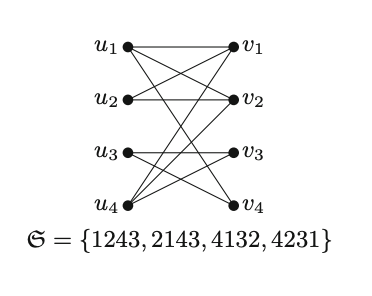
\includegraphics[width=7cm]{ex2}
	\caption{Đồ thị hai phía với $\mathfrak{S}$ là tập các ghép cặp hoàn hảo}
	\label{fig:image1}
\end{center}
\end{figure}
%$\sigma (\tau (1)), \sigma (\tau (2)), .... , \sigma (\tau (n))$
Ý tưởng của Radhakrishnan là xét các đỉnh  $u_{1}, u_{2}, ....  , u_{n}$ theo một \textit{thứ tự ngẫu nhiên $\tau \in S_{n}$}, trong đó mọi $\tau$ có xác suất như nhau và bằng $\frac{1}{n!}$, sau đó lấy giá trị trung bình của các entropy. Nói cách khác, ta xét các cặp ghép (\textit{matching}) theo thứ tự $\tau_{1},\tau_{2},..,\tau_{n}$ . Xét $\tau$ cố định, khi đó $k_{i} = \tau ^{-1}_{i}$ được hiểu là vị trí của $u_{i}$ theo thứ tự ngẫu nhiên $\tau$ là $k_{i}$. Khi đó, biểu thức \eqref{eqEntropy2} trở thành:
\begin{equation*}
	H(\sigma(1),...,\sigma(n)) = \displaystyle \sum_{i=1}^{n}H\Big(\sigma (i)| \sigma (\tau_{1}),...,\sigma (\tau_{k_{i}-1})\Big)
\end{equation*}
%H(\sigma(1),...,\sigma(n)) = \displaystyle \sum_{i=1}^{n}H(\sigma (i)| \sigma (\tau(1)),...,\sigma (\tau(k_{i}-1)))	
đúng với mọi $\tau$, lấy giá trị trung bình ta được: 
%\begin{equation*}
%	H(\sigma(1),...,\sigma(n)) = \frac{1}{n!}\displaystyle \sum_{\tau}\Bigg(\displaystyle \sum_{i=1}^{n}H(\sigma (i)| \sigma (\tau(1)),...,\sigma (\tau(k_{i}-1))) \Bigg)
%\end{equation*}
\begin{equation}
	H(\sigma(1),...,\sigma(n)) = \frac{1}{n!}\displaystyle \sum_{\tau}\Big(\displaystyle \sum_{i=1}^{n}H\Big(\sigma (i)| \sigma (\tau_{1}),...,\sigma (\tau_{k_{i}-1})\Big) \Big) \label{Hentropy}
\end{equation}

Xét biểu thức 
%\begin{equation}
%H(\sigma (i)| \sigma (\tau(1)),...,\sigma (\tau(k_{i}-1)))
%\end{equation}
\begin{equation}
H\Big(\sigma (i)| \sigma (\tau_{1}),...,\sigma (\tau_{k_{i}-1})\Big) \label{eqEntropy}
\end{equation}

Để tìm cận trên cho \eqref{eqEntropy}, ta sẽ sử dụng mệnh đề \textbf{(C)}, áp dụng với biến ngẫu nhiên $X=\Big( \sigma (\tau_{1}),...,\sigma (\tau_{k_{i}-1}) \Big)$ và $Y=\sigma(i)$. Với $\tau$ cố định $\in S_{n}$ và $\sigma \in \mathfrak{S}$, đặt $N_{i}(\sigma,\tau)$ là số các giá trị $k \in [n]$ sao cho $u_{i}v_{k} \in E(G)$ và k $\notin {\Big(\sigma(\tau_{1}),...,\sigma(\tau_{k_{i}-1}) \Big)}$ (nói cách khác, $N_{i}(\sigma,\tau)$ là số khả năng còn lại cho $\sigma(i)$ khi đã biết ($\sigma(\tau_{1}),...,\sigma(\tau_{k_{i}-1})$). Vì $deg(u_{i}) = d_{i}$  đồng thời $u_{i}$ phải được ghép cặp trong $\sigma$ nên $1 \leq N_{i}(\sigma,\tau) \leq d_{i} $ với mọi $\sigma \in \mathfrak{S}$. Tiến hành chia tập $supp X$ thành các tập con $E_{i,j}^{(\tau)}$ sao cho : 
\begin{equation*}
\Big(\sigma(\tau_{1}),...,\sigma(\tau_{k_{i}-1}) \Big) \in E_{i,j}^{(\tau)} <=> N_{i}(\sigma,\tau) = j, \textrm{ với } 1 \leq j \leq d_{i}
\end{equation*}
Coi $|N_{i}(\sigma,\tau)|$ là một biến ngẫu nhiên trên $\mathfrak{S}$, ta có:
\begin{equation*}
Pr(X \in  E_{i,j}^{(\tau)} ) = Pr( N_{i}(\sigma,\tau) = j)
\end{equation*}
Từ mệnh đề \textbf{(C)}, với $\tau$ cố định:
\begin{equation*}
\begin{array}{l@{}l}
H(\sigma (i)| \sigma (\tau_{1}),...,\sigma (\tau_{k_{i}-1})) 
    &{} \leq \displaystyle \sum_{j=1}^{d_{i}}Pr(N_{i}(\sigma,\tau)=j)\log_{2}j \\
    &{} = \displaystyle \sum_{j=1}^{d_{i}}\log_{2}j\displaystyle \sum_{\sigma \in \mathfrak{S}}P(\sigma).P(N_{i}(\sigma,\tau)=j | \sigma)  \textrm{ (Do } {\sigma \in \mathfrak{S}}  \textrm{ là 1 nhóm đầy đủ)}\\
    &{} = \displaystyle \sum_{j=1}^{d_{i}}\log_{2}j\displaystyle \sum_{\sigma \in \mathfrak{S}}\frac{P(N_{i}(\sigma,\tau)=j | \sigma)}{|\mathfrak{S}|}
\end{array}
\end{equation*}

Kết hợp với \eqref{Hentropy}
\begin{equation}
    H(\sigma (1),...,\sigma (n)) \leq \displaystyle \sum_{j=1}^{d_{i}}\log_{2}j \Bigg( \frac{1}{n!|\mathfrak{S}|} \displaystyle \sum_{\sigma \in \mathfrak{S}}\displaystyle \sum_{\tau \in S_{n}}P(N_{i}(\sigma,\tau)=j | \sigma) \Bigg)
\end{equation}


Xét $\displaystyle \sum_{\tau \in S_{n}}P(N_{i}(\sigma,\tau)=j | \sigma)$:\\
Với mỗi $\sigma$ cố định $\in \mathfrak{S}$, $N_{i}(\sigma,\tau)$ nhận các giá trị từ 1 tới $d_{i}$ với xác suất như nhau là $\frac{1}{d_{i}}$, vì $N_{i}(\sigma,\tau)$ chỉ phụ thuộc vào vị trí của $\sigma(i)$ trong hoán vị $\tau$ (do $\sigma$ đã cố định), tương ứng với các đỉnh $k$ thỏa mãn $u_{i}v_{k} \in E(G)$ (Nếu  $\sigma(i)$ là lân cận gần nhất của $i$ theo thứ tự của hoán vị (giả sử là $\tau_{1}$).  Khi đó $N_{i}(\sigma,\tau_{1}) = d_{i}$ và $P(N_{i}(\sigma,\tau_{1})=d_{i} | \sigma)=\frac{1}{d_{i}}$; Nếu  $\sigma(i)$ là lân cận gần thứ hai của $i$ theo thứ tự của hoán vị (giả sử $\tau_{2}$). Khi đó $N_{i}(\sigma,\tau_{2}) = d_{i}-1$ và $P(N_{i}(\sigma,\tau_{2})=d_{i}-1 | \sigma)=\frac{1}{d_{i}}$,...tương tự với n! hoán vị của $S_{n}$ .Do đó, giá trị của biểu thức trên bằng:
\begin{equation*}
    \displaystyle \sum_{\tau \in S_{n}}P(N_{i}(\sigma,\tau)=j | \sigma)=n!.\frac{1}{d_{i}} = \frac{n!}{d_{i}}
\end{equation*}
Và biểu thức \eqref{eqEntropy2} trở thành: 
\begin{equation*}
\begin{array}{l@{}l}
H(\sigma (1), \sigma (2), ....  ,\sigma (n)) 
&{}= \displaystyle \sum_{i=1}^{n}H(\sigma (i)| \sigma (1), \sigma (2), ....  ,\sigma (i-1)) \\
&{} \leq  \displaystyle \sum_{i=1}^{n}\displaystyle \sum_{j=1}^{d_{i}}\log_{2}j \Bigg(\frac{1}{n!|\mathfrak{S}|}\displaystyle \sum_{\sigma \in \mathfrak{S}}\frac{n!}{d_{i}} \Bigg) \\
 &{}= \displaystyle \sum_{i=1}^{n}\displaystyle \sum_{j=1}^{d_{i}}\log_{2}j \Bigg(\frac{1}{n!|\mathfrak{S}|}.|\mathfrak{S}|.\frac{n!}{d_{i}} \Bigg) \\
 &{}= \displaystyle \sum_{i=1}^{n}\displaystyle \sum_{j=1}^{d_{i}}\log_{2}j.\frac{1}{d_{i}} =\displaystyle \sum_{i=1}^{n}\frac{1}{d_{i}}\log_{2}(d_{i}!). 				\qedhere
\end{array}
\end{equation*}
\end{proof}
%$\sum_{i=1}^{n}\frac{1}{d_{i}}\log_{2}(d_{i}!).$
\chapter{Hình vuông Latin}
\section{Khái niệm}
Hình vuông latin là một trong số những hình tổ hợp lâu đời nhất, có những nghiên cứu rõ ràng từ thời cổ đại. Để có được hình vuông Latin, ta phải điền vào $n^{2}$ ô của một mảng các ô vuông kích thước $n \times n$ các số $1,2,..,n$ sao cho mỗi số điền vào chỉ xuất hiện đúng một lần ở mỗi hàng và mỗi cột chứa số đó. Nói cách khác, mỗi hàng và mỗi cột này là một hoán vị của tập $\{1,2,...,n\}$. Khi đó ta nói đó là hình vuông Latin bậc $n$.

\begin{table}[ht]
\centering
\begin{tabular}{|c|c|c|c|}
    \hline
     1&2&3&4  \\ \hline
     2&1&4&3  \\ \hline
     4&3&1&2  \\ \hline
     3&4&2&1  \\
     \hline
\end{tabular}
\caption{Hình vuông Latin bậc 4.}
\end{table}%

Ta xét bài toán: Xác định số hình vuông latin $L(n)$ bậc $n$. Xét một vài ví dụ nhỏ :\\
$n=1$:
\begin{tabular}{|c|}
    \hline
     1 \\ \hline
    
\end{tabular}: ~~~ $L(1) = 1$
\vspace{20pt}
\\
$n=2$:
\begin{tabular}{|c|c|}
    \hline
     1&2 \\ \hline
     2&1 \\ 
     \hline
\end{tabular} ~~~ \begin{tabular}{|c|c|}
    \hline
     2&1 \\ \hline
     1&2 \\ 
     \hline
\end{tabular}: ~~~ $L(2) = 2$
\vspace{20pt}
\\
$n=3$:
\begin{tabular}{|c|c|c|}
	\hline
	1&2&3 \\ \hline
	2&3&1 \\ \hline
	3&1&2 \\
	\hline
\end{tabular}: ~~~ $L(3) = 12$

\begin{equation*}
L(1) = 1, L(2) = 2, L(3) = 12, L(4) = 576, L(5) = 161280
\end{equation*}
Ta thấy khi n lớn, thì số lượng hình vuông Latin bậc n tăng rất nhanh. Liệu ta có thể tìm được một chặn trên cho giá trị này ? Kết quả của định lý Brégman sẽ giải quyết được vấn đề này.
\section{Mô hình bài toán}
Xét một hình vuông $n \times n$ và điền vào đó các số $1,2,..,n$ sao cho đó là một hình vuông Latin. Có $n!$ cách điền vào hàng đầu tiên (hoán vị của $n$ phần tử). Giả sử $n-k$ hàng đầu tiên đã được điền và cho ta một hình chữ nhật Latin R kích thước $(n-k) \times n$. Vậy có bao nhiêu cách để điền vào hàng tiếp theo? Xét một đồ thị hai phía $G_k = (U \cup V,E)$, trong đó $U$ là tập các phần tử $\{1,2,..,n\}$ và $V$ là tập các vị trí của cột, sao cho:
\begin{equation*}
ij \in E :\Leftrightarrow i \textrm{ không xuất hiện trong cột thứ } j \textrm{ của } R.
\end{equation*}
Nói cách khác, một cách điền phù hợp trong hàng tiếp theo tương ứng với một cặp ghép hoàn hảo (\textit{perfect matching}) trong đồ thị hai phía $G_k = (U \cup V,E)$. Bây giờ, mọi thành phần $i \in U$ xuất hiện $n-k$ lần trong $R$ nên nó sẽ xuất hiện trong $k$ cột còn lại của hàng tiếp theo. Do đó, $i$ có bậc $k$ trong $G_k$ và tương tự $d(j) = k $ với $j \in V$. \\
%\begin{figure}
%\begin{center}
%	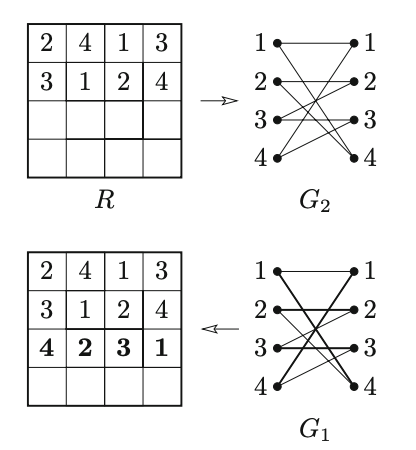
\includegraphics[width=7cm]{ex3}
%%	\caption{Đồ thị hai phía với $\mathfrak{S}$ là tập các perfect matching}
%\end{center}
%\end{figure}
\begin{center}
	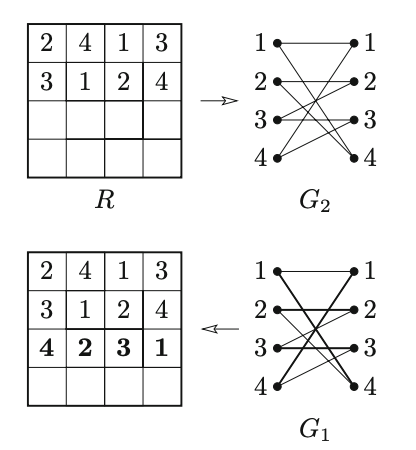
\includegraphics[width=7cm]{ex3}
%	\caption{Đồ thị hai phía với $\mathfrak{S}$ là tập các perfect matching}
\end{center}
Đặt $M_k$ là ma trận $0/1$ tương ứng với $G_k$, khi đó:
\begin{equation*}
	\textrm{per } M_k = \textrm{số cách điền phù hợp của hàng } n-k+1.
\end{equation*}
Mọi hàng và cột trong $M_k$ có tổng bằng $k$; ta kí hiệu tập các ma trận $0/1$ bởi $\mathcal{M}(n,k)$. Giá trị $per$ $M_k$ phụ thuộc vào việc sắp xếp ma trận R, nhưng nếu ta có một cận trên và cận dưới hợp lý cho các ma trận trong $\mathcal{M}(n,k)$, khi ta lấy tích trên các giá trị của $k$, ta thu được một cận trên/cận dưới cho $L(n)$.\\
Sử dụng định lý Brégman với $d_1=d_2=...=d_n=k$ ta có ngay
\begin{equation*}
	\textrm{per } M \leq k!^{\frac{n}{k}}		 \textrm{								với mọi      }M \in \mathcal{M}(n,k)
\end{equation*} 
Bây giờ là giá trị cho cận dưới: Giả sử $k<n$ và đặt $L$ là hình chữ nhật Latin $k \times n$ ($k$ hàng trên đã được điền) trên $\{1,2,...,n\}$. Để tính số cách điền các số vào các hàng tiếp theo ($k+1$) để tạo thành hình chữ nhật Latin $(k+1) \times n$, đặt $M=(m_{ij})$ là một ma trận sao cho $m_{ij} = 1$ nếu $i$ không xuất hiện ở cột thứ $j$ và bằng $0$ nếu ngược lại. Khi đó giá trị $\textrm{per }(M)$ sẽ đếm số cách có thể điền vào hàng thứ $k+1$. Tổng theo hàng và cột của ma trận $M = n-k$ nên $\frac{1}{n-k}B$ là ma trận \textit{ngẫu nhiên kép}. Theo định lý \eqref{eqPer} về vĩnh thức: $\textit{per }(M) \geq (n-k)^n\frac{n!}{n^n}$ nên ta có:
\begin{equation*}
	L(n) \geq n! \displaystyle\prod_{k=1}^{n-1}\{ (n-k)^{n}\frac{n!}{n^n} \} = \frac{(n!)^{2n}}{n^{n^2}} .
\end{equation*}
% Nếu $M$ nằm trong $\mathcal{M}(n,k)$ thì $\frac{1}{k}M$ là ma trận \textit{doubly stochastic}. Theo định lý về vĩnh thức (....) 
%\begin{equation*}
%	\textrm{per }M = k^{n}\textrm{per}\Big( \frac{1}{k}M \Big) \geq k^{n}\frac{n!}{n^n}
%\end{equation*}
Tổng quát, ta đã chứng minh được kết quả đáng chủ ý sau:
\begin{theorem}
	Số hình vuông Latin bậc n (kí hiệu: L(n)) thoả mãn
	\begin{equation*}
		\frac{n!^{2n}}{n^{n^2}} \leq L(n) \leq \displaystyle \prod_{k=1}^{n} k!^{\frac{n}{k}}.
	\end{equation*}
\end{theorem}

Sử dụng tính xấp xỉ của $n!$:
\begin{equation}
	\Big( \frac{n}{e} \Big)^n < n! < en\Big(\frac{n}{e} \Big)^n, \label{n!}
\end{equation}
Ta có thể rút ra công thức về giới hạn sau đây.

\begin{corollary}
	Theo giới hạn, số hình vuông Latin bậc $n$, kí hiệu bởi $L(n)$ thoả mãn
	\begin{equation*}
		\lim_{n \to \infty} \frac{L(n)^{\frac{1}{n^2}}}{n} = \frac{1}{e^2}
	\end{equation*}
\end{corollary}
\begin{proof}
	Từ cận dưới của $L(n)$ ta có
	\begin{equation*}
		L(n) \geq \frac{n!^{2n}}{n^{n^2}} > \frac{\Big( \frac{n}{e}\Big)^{2n^2}}{n^{n^2}} = \Big(\frac{n}{e^2} \Big)^{n^2}
	\end{equation*}
	nên $\frac{L(n)^{\frac{1}{n^2}}}{n} > \frac{1}{e^2}$ và do đó $\displaystyle \lim_{n \to \infty} \frac{L(n)^{\frac{1}{n^2}}}{n} \geq \frac{1}{e^2}$ \\
	Để tìm cận trên, ta sẽ chỉ ra với mọi $\epsilon > 0$,
		\begin{equation*}
			\frac{L(n)^{\frac{1}{n^2}}}{n}  < \frac{1}{e^2}(1+\epsilon)
		\end{equation*}
		đúng khi $n$ đủ lớn. Để thuận tiện ta đặt $\mathcal{L}(n) = L(n)^{\frac{1}{n^2}}. $
		Sử dụng \eqref{n!} , ta có
		\begin{equation*}
		\begin{array}{l@{}l}

			\log\mathcal{L}(n)
			&{} \leq \frac{1}{n}\log \displaystyle \prod_{k=1}^{n}(k!)^{\frac{1}{k}} = \frac{1}{n} \displaystyle \sum_{k=1}^{n}\frac{1}{k}\log k! \\ 
			&{} < \frac{1}{n}\displaystyle \sum_{k=1}^{n}\frac{1}{k}\log\Big( ek \Big(\frac{k}{e}\Big)^{k} \Big) \\
			&{} = \frac{1}{n} \displaystyle \sum_{k=1}^{n}\frac{1}{k}(1 +\log k + k\log k -k) \\
			&{} = \frac{1}{n} \Big[\displaystyle \sum_{k=1}^{n}\frac{1}{k} + \displaystyle \sum_{k=1}^{n}\frac{\log k}{k} + \displaystyle \sum_{k=1}^{n}\log k -n \Big].
		\end{array}
		\end{equation*}
		Trong đó tổng đầu tiên là số $Harmonic$ $H_n$: $H_n < \log n +1$. Tổng thứ 3 được đánh giá thông qua \eqref{n!}, với:
		\begin{equation}
			\displaystyle \sum_{k=1}^{n} \log k < \log\Big( en\Big(\frac{n}{e}\Big)^{n}\Big) = 1+ (n+1)\log n -n \leq (n+2 )\log n - n \label{eq}
		\end{equation}
		Đối với tổng thứ hai, vì $\frac{\log x}{x}$ luôn dương với mọi $x>1$ và là hàm đơn điệu giảm với $x >e$, ta có:
		\begin{equation*}
			\int_{1}^{n}\frac{\log x}{x} \geq \displaystyle \sum_{k=4}^{n}\int_{k-1}^{k}\frac{\log x}{x}dx \geq \displaystyle \sum_{k=4}^{n}\int_{k-1}^{k}\frac{\log k}{k}dx = \displaystyle \sum_{k=4}^{n}\frac{\log k}{k},
		\end{equation*}
		nên 
		\begin{equation}
			 \displaystyle \sum_{k=1}^{n}\frac{\log k}{k} \leq 2 + \Big[\frac{1}{2}(\log x)^2\Big] \Big|_1^n  = 2+ \frac{1}{2}(\log n)^2. \label{eq1}
		\end{equation}
Từ \eqref{eq} và \eqref{eq1} ta có: 
\begin{equation*}
	\log \mathcal{L}(n) < \frac{3\log n}{n} + \frac{3}{n} + \frac{(\log n)^2}{2n} + \log n -2,
\end{equation*}
trong đó 3 số hạng đầu tiến dần về 0 khi n đủ lớn. Do đó, với mọi $\delta >0$:
\begin{equation*}
	\log \mathcal{L}(n) \leq \delta +\log n -2 .
\end{equation*}
nên $L(n)^\frac{1}{n^2} \leq \frac{n}{e^2}e^{\delta}$ khi $n$ đủ lớn. Ta có điều phải chứng minh.
\end{proof}


\chapter*{TỔNG KẾT}
\addcontentsline{toc}{chapter}{Tổng kết} 
\mdseries

	Qua bài báo cáo này, em đã tìm hiểu được một trong những đặc trưng của ma trận là vĩnh thức,  cùng với chứng minh các bất đẳng thức liên quan đến giá trị này thông qua các phép biến đổi đại số và kiến thức về entropy từ lý thuyết thông tin, qua đó ứng dụng chúng để giải quyết bài toán đếm tổ hợp xác định số hình vuông Latin bậc $n$.

%	Một lần nữa khằng định, phương pháp phân tích thành phần chính là phương pháp giảm chiều dữ liệu hiệu quả nhất. PCA thực chất là đi tìm một phép xoay tương ứng với một ma trận trực giao sao cho trong hệ toạ độ mới, tồn tại các chiều có phương sai nhỏ mà ta có thể bỏ qua; ta chỉ cần giữ lại các chiều/thành phần khác quan trọng hơn. Như đã chứng minh ở trên, tổng phương sai theo mọi chiều trong hệ cơ sở nào cũng là như nhau và bằng tổng các trị riêng của ma trận hiệp phương sai. Vì vậy, PCA còn được coi là phương pháp giảm số chiều dữ liệu mà giữ được tổng phương sai còn lại là lớn nhất.
	





%$\sigma (\tau_{1}), \sigma (\tau_{2}), .... , \sigma (\tau_{n})$
%
%$H(\sigma (\tau_{1}),..,\sigma (\tau_{n})) = \displaystyle \sum_{i=1}^{n}H(\sigma (\tau_{i})| \sigma (\tau_{1}),...,\sigma (\tau_{k_{i}-1}))$
%
%$H(\sigma (\tau_{1}),..,\sigma (\tau_{n})) = \frac{1}{n!}\displaystyle \sum _{\tau}\left ( \displaystyle \sum_{i=1}^{n}H(\sigma (\tau_{i})| \sigma (\tau_{1}),...,\sigma (\tau_{k_{i}-1})) \right )$
%
%$\Theta(n^{\log_2 2} )$
\chapter*{Tài liệu tham khảo}
\addcontentsline{toc}{chapter}{Tài liệu tham khảo}
\mdseries
\begin{itemize}
\item[1.]
	Martin Aigner, Günter M. Ziegler, ‘‘Proofs from THE BOOK’’, $6^{th}$ Edition.
\item[2.]
	Valle Martinez, Vicente, "Notes on the proof of the van der Waerden permanent conjecture" (2018).
\end{itemize}
\end{document}